%%
%% This is file `sample-acmlarge.tex',
%% generated with the docstrip utility.
%%
%% The original source files were:
%%
%% samples.dtx  (with options: `acmlarge')
%% 
%% IMPORTANT NOTICE:
%% 
%% For the copyright see the source file.
%% 
%% Any modified versions of this file must be renamed
%% with new filenames distinct from sample-acmlarge.tex.
%% 
%% For distribution of the original source see the terms
%% for copying and modification in the file samples.dtx.
%% 
%% This generated file may be distributed as long as the
%% original source files, as listed above, are part of the
%% same distribution. (The sources need not necessarily be
%% in the same archive or directory.)
%%
%%
%% Commands for TeXCount
%TC:macro \cite [option:text,text]
%TC:macro \citep [option:text,text]
%TC:macro \citet [option:text,text]
%TC:envir table 0 1
%TC:envir table* 0 1
%TC:envir tabular [ignore] word
%TC:envir displaymath 0 word
%TC:envir math 0 word
%TC:envir comment 0 0
%%
%%
%% The first command in your LaTeX source must be the \documentclass
%% command.
%%
%% For submission and review of your manuscript please change the
%% command to \documentclass[manuscript, screen, review]{acmart}.
%%
%% When submitting camera ready or to TAPS, please change the command
%% to \documentclass[sigconf]{acmart} or whichever template is required
%% for your publication.
%%
%%
\documentclass[acmlarge]{acmart}
\usepackage{lipsum}
%\usepackage{amsmath}
%\usepackage{amssymb}
%\usepackage{graphicx}
\usepackage[linesnumbered]{algorithm2e}
\usepackage{enumitem}

\usepackage{listings}% http://ctan.org/pkg/listings
\lstset{
  basicstyle=\ttfamily,
  mathescape
}

%%
%% \BibTeX command to typeset BibTeX logo in the docs
\AtBeginDocument{%
  \providecommand\BibTeX{{%
    Bib\TeX}}}

%% Rights management information.  This information is sent to you
%% when you complete the rights form.  These commands have SAMPLE
%% values in them; it is your responsibility as an author to replace
%% the commands and values with those provided to you when you
%% complete the rights form.
\setcopyright{acmcopyright}
\copyrightyear{2022}
\acmYear{2022}
\acmDOI{XXXXXXX.XXXXXXX}


%%
%% These commands are for a JOURNAL article.
\acmJournal{POMACS}
\acmVolume{37}
\acmNumber{4}
\acmArticle{111}
\acmMonth{8}

%%
%% Submission ID.
%% Use this when submitting an article to a sponsored event. You'll
%% receive a unique submission ID from the organizers
%% of the event, and this ID should be used as the parameter to this command.
%%\acmSubmissionID{123-A56-BU3}

%%
%% For managing citations, it is recommended to use bibliography
%% files in BibTeX format.
%%
%% You can then either use BibTeX with the ACM-Reference-Format style,
%% or BibLaTeX with the acmnumeric or acmauthoryear sytles, that include
%% support for advanced citation of software artefact from the
%% biblatex-software package, also separately available on CTAN.
%%
%% Look at the sample-*-biblatex.tex files for templates showcasing
%% the biblatex styles.
%%

%%
%% The majority of ACM publications use numbered citations and
%% references.  The command \citestyle{authoryear} switches to the
%% "author year" style.
%%
%% If you are preparing content for an event
%% sponsored by ACM SIGGRAPH, you must use the "author year" style of
%% citations and references.
%% Uncommenting
%% the next command will enable that style.
%%\citestyle{acmauthoryear}


%%
%% end of the preamble, start of the body of the document source.
\begin{document}

%%
%% The "title" command has an optional parameter,
%% allowing the author to define a "short title" to be used in page headers.
\title{CSE6140 Final Project}

%%
%% The "author" command and its associated commands are used to define
%% the authors and their affiliations.
%% Of note is the shared affiliation of the first two authors, and the
%% "authornote" and "authornotemark" commands
%% used to denote shared contribution to the research.
\author{Avery Bodenstein}
\authornote{All authors contributed equally to this research.}
\email{abodenstein3@gatech.edu}
\affiliation{%
  \institution{Georgia Institute of Technology}
  \streetaddress{North Ave NW}
  \city{Atlanta}
  \state{Georgia}
  \country{USA}
  \postcode{30332}
}

\author{Adrian Thinnyun}
\authornotemark[1]
\affiliation{%
	\institution{Georgia Institute of Technology}
	\streetaddress{North Ave NW}
	\city{Atlanta}
	\state{Georgia}
	\country{USA}
	\postcode{30332}
}

\author{Jai Jacob}
\authornotemark[1]
\affiliation{%
	\institution{Georgia Institute of Technology}
	\streetaddress{North Ave NW}
	\city{Atlanta}
	\state{Georgia}
	\country{USA}
	\postcode{30332}
}

\author{Zheyi Zhang}
\authornotemark[1]
\affiliation{%
	\institution{Georgia Institute of Technology}
	\streetaddress{North Ave NW}
	\city{Atlanta}
	\state{Georgia}
	\country{USA}
	\postcode{30332}
}


%%
%% The abstract is a short summary of the work to be presented in the
%% article.
\begin{abstract}
  % A clear and well-documented \LaTeX\ document is presented as an
  % article formatted for publication by ACM in a conference proceedings
  % or journal publication. Based on the ``acmart'' document class, this
  % article presents and explains many of the common variations, as well
  % as many of the formatting elements an author may use in the
  % preparation of the documentation of their work.
  In this project, we implement and evaluate four different algorithms for solving the Minimum Vertex Cover problem: a branch and bound algorithm, a construction heuristic algorithm, a simulated annealing algorithm, and a genetic algorithm. We found that the construction heuristic algorithm achieved the overall best performance in terms of time and quality of solutions produced, with the branch and bound algorithm failing to improve upon the heuristic solution before the time cutoff and the local search algorithms incurring greater runtime and producing solutions of lower quality.
\end{abstract}

%%
%% The code below is generated by the tool at http://dl.acm.org/ccs.cfm.
%% Please copy and paste the code instead of the example below.
%%
\begin{CCSXML}
	<ccs2012>
	<concept>
	<concept_id>10003752.10003809.10003635</concept_id>
	<concept_desc>Theory of computation~Graph algorithms analysis</concept_desc>
	<concept_significance>500</concept_significance>
	</concept>
	<concept>
	<concept_id>10003752.10003809.10011254.10011256</concept_id>
	<concept_desc>Theory of computation~Branch-and-bound</concept_desc>
	<concept_significance>500</concept_significance>
	</concept>
	<concept>
	<concept_id>10003752.10003809.10003636</concept_id>
	<concept_desc>Theory of computation~Approximation algorithms analysis</concept_desc>
	<concept_significance>500</concept_significance>
	</concept>
	</ccs2012>
\end{CCSXML}

\ccsdesc[500]{Theory of computation~Graph algorithms analysis}
\ccsdesc[500]{Theory of computation~Branch-and-bound}
\ccsdesc[500]{Theory of computation~Approximation algorithms analysis}

%%
%% Keywords. The author(s) should pick words that accurately describe
%% the work being presented. Separate the keywords with commas.
\keywords{minimum vertex cover, spanning, topology, heuristics}

\received{4 December 2022}

%%
%% This command processes the author and affiliation and title
%% information and builds the first part of the formatted document.
\maketitle

\section{Introduction}

% short summary of the problem, the approach and the results you have obtained

The Minimum Vertex Cover (MVC) problem is a classical NP-complete problem with a wide variety of real-world and theoretical applications. The problem consists of finding the smallest subset of vertices in a graph that includes at least one endpoint of every edge in the graph. It is the optimization version of the Vertex Cover problem, which instead asks if there exists a subset of vertices of size less than or equal to a given positive integer that includes at least one endpoint of every edge in the graph.

The problem is in NP, meaning that a solution to the problem cannot be found with an algorithm that runs in polynomial time if P $\neq$ NP. Moreover, the problem is in NP-hard, meaning that every problem in NP is polynomially reducible to MVC (i.e. any instance of an NP problem can be converted into an instance of MVC in polynomial time). Since MVC is both in NP and NP-hard, it is also NP-complete, and was included as one of Karp's original 21 NP-complete problems \cite{karp1972reducibility}.

In this project, we implemented and tested four different approaches to the Minimum Vertex Cover problem. The first approach is a branch and bound (BnB) algorithm which runs in exponential time in the worst-case but may perform significantly better than a brute force search and is guaranteed to provide an optimal solution. The second approach is a construction heuristic algorithm, in particular the \textit{Greedy Independent Cover (GIC)} algorithm proposed by Halld\'{o}rsson and Radhakrishnan \cite{Hall97}, which runs in polynomial time and produces a solution with an approximation guarantee. The final two approaches are local search algorithms which run in polynomial time and produce solutions without a guarantee of quality. The first local search algorithm is based on simulated annealing, and the other is based on a genetic algorithm.

Overall, we found that the construction heuristic algorithm exhibited the best performance, both in terms of runtime and quality of solution produced. The algorithm ran much faster than either of the two local search algorithms tested and produced solutions with very low relative error compared to the optimal solution. 


\section{Problem Definition}

Given a graph $G = (V,E)$, a vertex cover of $G$ is a subset of vertices $A \subseteq V$ such that for every edge $(u,v) \in E$, $u \in A \lor v \in A$. The Minimum Vertex Cover problem is then the problem of finding a vertex cover $S$ of $G$ such that for every vertex cover $A$ of $G$, $|S| \leq |A|$, i.e. $S$ is the smallest vertex cover of $G$. In other words, the problem consists of finding a vertex cover of $G$ using as few vertices as possible.

\section{Related Work}

% a short survey of existing work on the same problem, and important results in theory and practice

The Vertex Cover problem was introduced in Karp's 21 NP-complete problems as the "Node Cover" problem \cite{karp1972reducibility}. The problem was defined as follows:
\begin{lstlisting}
NODE COVER
INPUT: graph G', positive integer l
PROPERTY: There is a set R $\subseteq$ N' such that |R| $\subseteq$ l and
every arc is incident with some node in R.
\end{lstlisting}

As part of Karp's result that the Satisfiability problem is reducible to each of the other problems listed in the paper, he showed that the Clique problem is reducible to the Node Cover problem, and that the Node Cover problem is reducible to the Feedback Node Set problem, the Feedback Arc Set problem, the Directed Hamilton Circuit problem, and the Set Covering problem.

Since its introduction, the Minimum Vertex Cover problem has had a wide range of theoretical and practical results related to it. In 1983, Bar-Yehuda and Even \cite{bar1983local} presented an algorithm that produces a solution to the problem with an approximation ratio of $2-\Theta(\frac{\log \log n}{\log n})$. A similar result was achieved by Monien and Speckenmeyer \cite{monien1985ramsey}.  
With $\Delta$ as the maximal degree of the graph, Hochbaum \cite{hochbaum1983efficient} was able to approximate the problem with a ratio of $(2 - \frac{2}{\Delta})$. This result was improved by Halld\'{o}rsson and Radhakrishnan \cite{Hall97} whose algorithm achieves an approximation ratio of $2- \frac{\log \Delta + O(1)}{\Delta}$, and then again by Halperin \cite{halperin2002improved} who achieved an approximation ratio of $(2 - (1 - o(1)) \frac{2 \ln \ln \Delta}{\ln \Delta})$ by using semidefinite programming relaxations. This result was improved further by Karakostas \cite{karakostas2005better} who used an even stronger semidefinite programming relaxation to achieve an approximation ratio of $2 - \Theta (\frac{1}{\sqrt{\log n}})$.

Several local search algorithms have been proposed for the Minimum Vertex Cover problem. One such algorithm is Edge Weighting Local Search (EWLS) \cite{cai2010ewls}, which is an iterated search algorithm based on the idea of extending a partial vertex cover into a full vertex cover. Another algorithm proposed for MVC is NuMVC \cite{cai2013numvc}, which uses a two-stage exchange strategy and edge weighting with forgetting to improve upon state-of-the-art algorithms. A stochastic local search algorithm named COVER (Cover Edges Randomly) \cite{richter2007stochastic}, which combines several heuristic criteria and a healthy dose of randomness to strike a balance between guided search and diversity.

\section{Algorithms}

%Detailed description of each algorithm you have implemented, with pseudo-code, approximation guarantee (if any), time and space complexities, etc. What are the potential strengths and weaknesses of each type of approach? Did you use any kind of automated tuning or configuration for your local search? Why and how you chose your local search approaches and their components? Please cite any sources of information that you used to inform your algorithm design

The algorithms implemented in this project fall under one of three major paradigms. The first is the Branch and Bound paradigm which constructs solutions one element at a time and prunes candidates from the search tree if the lower bound of their solution quality is worse than that of the current best solution seen. The second is the Approximation paradigm, in which the runtime of the algorithm is prioritized and optimized for by allowing the quality of the resulting solution to be worse than that of the optimal one up to a specified ratio. The last is the Local Search paradigm which starts at an initial point in the search space and iteratively traverses to neighboring points according to a specified evaluation function. Within this paradigm we chose to 

\subsection{Branch and Bound}

\subsubsection{Description}

The branch and bound approach is a non-polynomial time algorithm which is guaranteed to return an optimal solution. The BnB algorithm at worst does not perform any better than a brute force search, but can have significant performance gains where portions of the search space can be pruned. This pruning is performed by iteratively defining sub-problems and determining lower bounds on the cost to go for these sub-problems. If the best possible cost for a sub-problem exceeds the current best cost that subproblem (and therefore all it's derivatives) can be pruned from the search space. The sub-problems presented in this algorithm are defined based on inclusion or exclusion of nodes from the cover set. 

\newpage
\subsubsection{Pseudo Code}

-\\

The overall branch and bound algorithm has the following structure:\\

\begin{algorithm}[H]
	\caption{Branch and Bound}
	\SetAlgoLined
	\KwData{P}
	
	$F \leftarrow {(\emptyset,P)}$\;
	$B \leftarrow {(+\infty,(\emptyset,P))}$\;
	\While{F not empty}{
		choose $(X,Y)$ in F\;
		expand $(X,Y)$\;
		let $(x_1,y_1)$, $(x_2,y_2)$ be new configurations\;
		\ForEach{$(x_i,y_i)$}{
			\If{solution found}{
				\If{cost($x_i$) $<$ B}{
					$B \leftarrow ($cost$(x_i),(x_i,y_i))$\;
				}
			}
			\If{not dead end}{
				\If{lowerBound($x_i$) $<$ B}{
					$F \leftarrow F \cup {(x_i,y_i)}$\;
				}
			}
		}
	}
	
	return (B)
\end{algorithm}

where P is the graph, $x_i$ are all the vertices in the cover set, and $y_i$ are the vertices remaining for selection. There are four sub functions, "choose", "expand", "checkSolution", "checkDeadEnd", and "lowerBound". In the implementation presented here, choose selects the subproblem in F with the lowest lowerBound on cost to go. Expand takes that subproblem and returns two subproblems, one with the node with fewest unique edges selected and one without that node as a possible selection. checkSolution checks to see if all edges are covered by $x_i$. checkDeadEnd checks if $x_i \cup y_i$ covers all edges. Finally lowerBound runs the heuristic algorithm described in this report on $y_i$ then divides by the approximation ratio (2) to get a lower bound on the possible additional nodes required to cover all edges. This is then added to the number of nodes already in $x_i$.




\subsubsection{Algorithm Analysis}

% Additional description\\

% Gives exact solution\\

% Time and space complexity\\

The primary strength of the branch and bound algorithm is that, with sufficient time and computation, it will return the exact, optimal solution. This feature of the algorithm distinguishes it from the other three algorithms tested, each of which either provides a solution with an approximation guarantee or a solution with no guarantees whatsoever regarding its quality. Additionally, the branch and bound algorithm can often perform much better and consume far less time/space than a brute-force search if it manages to prune large sections of the search tree during its bounding operations.

The main downside of the branch and bound algorithm is of course that the worst-case time/space complexity of the algorithm is still exponential, i.e. $O(2^n)$ where $n$ is the number of nodes. While ideally the introduction of the lower bound would allow the algorithm to prune large parts of the search tree, in practice the algorithm may take just as long as a brute-force search to find the optimal solution.

\subsection{Construction Heuristic}

\subsubsection{Description}

The construction heuristic approach implemented here is the \textit{Greedy Independent Cover (GIC)} algorithm, presented in Halld\'{o}rsson and Radhakrishnan [1994] \cite{Hall97} for the independent set problem. This is an approximation approach which runs in polynomial time and yields an answer within a bound of the optimal solution. Runtime and Approximation Ratio analysis is provided in \ref{app_alg_analy}. This algorithm lends itself well to use with priority queues. All vertices in the graph are stored in a priority queue, ordered by the number of adjacent edges remaining in G: q[nodeLabel] = [nEdges,destinationNodes]. At each iteration the vertex with the fewest remaining edges is popped from the queue. Each of it's neighbors is then removed from the queue and added to the cover set. For each remaining edge in each neighbor, the source node is removed from the list of edges in the destination node and the number of edges in the destination node is lowered by one. This process continues until all edges are covered.

\subsubsection{Pseudo Code}

-\\

\begin{algorithm}[H]
	\caption{Greedy Independent Cover (GIC)}
	\SetAlgoLined
	\KwData{G = (V,E)}
	C $\leftarrow$ $\emptyset$\;
	\While{$E \not= \emptyset$ }
	{
		select a vertex u of minimum degree\;
		C $\leftarrow$ C $\cup$ N(u)\;
		V $\leftarrow$ V - (N(u) $\cup$ {u})\;
	}
	\Return C\;
\end{algorithm}

Where N(u) is the neighborhood (all adjacent vertices to) u.\\

\begin{algorithm}[H]
	\caption{Detailed Implementation}
	\SetAlgoLined
	\KwData{q,nEdges}
	C $\leftarrow$ 0\;
	\While{$C <$ nEdges }
	{
		u $\leftarrow$ q.peek()\;
		\ForEach{neigbor i in N(u)}{
			C $\leftarrow$ C + {q[i][0]}\;
			\ForEach{edge (i,j) in neighbor}{
				q[j][0] $\leftarrow$ q[j][0] - 1\;
				q[j][1] $\leftarrow$ q[j][1] - $\{i\}$\;
			}
		} 
		q = q - u\;
	}
	\Return C\;
\end{algorithm}

\subsubsection{Algorithm Analysis}\label{app_alg_analy}

-\\

As discussed in Delbot and Laforest [2010] \cite{Fran10} the Greedy Independent Cover algorithm performs extremely well. As can be seen in table \ref{table:alg_perf} the relative error for GIC never exceeds 6\% (and this is on the Jazz graph where the estimated solution is only 1 node larger than the optimal solution). However, the disadvantage of GIC is that the worst case performance is relatively poor. As shown in Avis and Imamura [2007] \cite{Avis06}, the approximation ratio is at least $\frac{\sqrt{\Delta}}{2}$ where $\Delta$ is the maximum degree in G.

Figure \ref{fig:approx_comp} shows a comparison between the approximation ratios of several common algorithms described in \cite{Fran10}. Note that while GIC performs quite well, its approximation ratio exceeds Depth First Search, or either of the Edge Deletion bounds for any $\Delta$ above 16.

\begin{figure}[h]
	\centering
	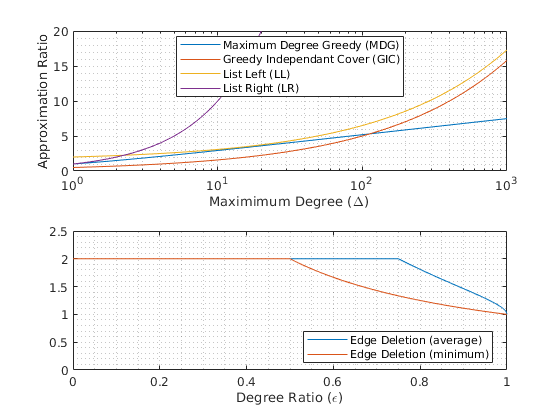
\includegraphics[width=0.8\linewidth]{ApproxRatioComp.png}
	\caption{Comparison of approximation ratios between several Vertex Cover heuristics}
	\Description{Comparison of approximation ratios between several Vertex Cover heuristics}
	\label{fig:approx_comp}
\end{figure}



The time complexity of the GIC algorithm as implemented is $O(n^2)$ where n is the number of nodes. As each node is selected via the minimum cardinality, at worst it has zero neighbors, so there would be at worst $n$ node selections. However in this case there would be 0 edge updates. For every neighbor that is present there are edge updates equal to the neighbors' cardinality. This can be at most $n-i$, where $i$ is the number of previous node selections. The complete complexity is then $O(\frac{n}{2}(n+1))$.

\subsection{Local Search 1 (Simulated Annealing)}

\subsubsection{Description}

The first local search algorithm we implemented is simulated annealing. The main task is to find an appropriate cost evaluation function, and to define the neighborhood.

For the first question, we define the cost as $$|V'|+\alpha\; \texttt{number of edges uncovered}$$ 
In the equation, $\alpha$ is a factor that defines how important it is to cover all the edges while exploring new solutions. Then the main procedure is to start with an initial solution with a greedy algorithm and a large temperature, lower it gradually in each loop, find a neighbor and evaluate it, choose to switch to it or not using the probability given the evaluated cost change.

For the second question, we define a neighbor in this algorithm as a set of vertices that differ from the current set with exactly one vertex, that is, the neighbor either has one more vertex in the set, or has all but one vertex compared with the current one. Using this definition, we can possibly go to the optimal solution in the sense that it is connected to the initial solution via the neighbor relationship.

\subsubsection{Pseudo Code}

-\\

The simulated annealing algorithm has the following structure:\\

\begin{frame}{}
  \begin{center}
    \scalebox{0.8}{
    \begin{minipage}{0.7\linewidth}
      \begin{algorithm}[H]
	\caption{Simulated Annealing}
	\SetAlgoLined
	\KwData{V,E}
	$init\_sol$ = init(V, E, neighbors)\;
	$best$ = (len($init\_sol$), $init\_sol$)\;
	$v\_set = init\_sol$\;
	$edges$ = edges covered by $v\_set$\;
	T = $T_{max}$\;
	\While{T $> 0$}
	{
		$next$ = random\_of($\{1,2,\dots,|V|\}$)\;
		$gain$ = 0\;
		\If{$next \in v\_set$}
		{
			$gain += 1$\;
			\For{$j \in neighbors[next]$}
			{
				\If{$j\notin v\_set$}{$gain -= \alpha$}
			}
		}
		\Else
		{
			$gain -= 1$\;
			\For{$j \in neighbors[next]$}
			{
				\If{$j\notin v\_set$}{$gain += \alpha$}
			}
		}
		$p = \min\{1, e^{\frac{gain}{T}}\}$\;
		\If{random(0,1) < $p$}
		{
			\If{$next \in v\_set$}
			{
				$v\_set$.remove($next$)\;
				\For{$j \in neighbors[next]$}
				{
					\If{$j\notin v\_set$}{edges.remove($next, j$)}\;
				}
			}
			\Else
			{
				$v\_set$.add($next$)\;
				\For{$j \in neighbors[next]$}
				{
					\If{$j\notin v\_set$}{edges.add($next, j$)}
				}
			}
		}
		\If{len($edges$) == $|E|$ \textbf{and} len($v\_set$)<$best[0]$}{$best = (len(v\_set), v\_set)$}
		$T -= T_{MAX}/k$\;
	}
	return ($best$)
\end{algorithm}
    \end{minipage}%
    }
  \end{center}

\end{frame}

% \begin{algorithm}[H]
% 	\caption{Simulated Annealing}
% 	\SetAlgoLined
% 	\KwData{V,E}
% 	$init\_sol$ = init(V, E, neighbors)\;
% 	$best$ = (len($init\_sol$), $init\_sol$)\;
% 	$v\_set = init\_sol$\;
% 	$edges$ = edges covered by $v\_set$\;
% 	T = $T_{max}$\;
% 	\While{T $> 0$}
% 	{
% 		$next$ = random\_of($\{1,2,\dots,|V|\}$)\;
% 		$gain$ = 0\;
% 		\If{$next \in v\_set$}
% 		{
% 			$gain += 1$\;
% 			\For{$j \in neighbors[next]$}
% 			{
% 				\If{$j\notin v\_set$}{$gain -= \alpha$}
% 			}
% 		}
% 		\Else
% 		{
% 			$gain -= 1$\;
% 			\For{$j \in neighbors[next]$}
% 			{
% 				\If{$j\notin v\_set$}{$gain += \alpha$}
% 			}
% 		}
% 		$p = \min\{1, e^{\frac{gain}{T}}\}$\;
% 		\If{random(0,1) < $p$}
% 		{
% 			\If{$next \in v\_set$}
% 			{
% 				$v\_set$.remove($next$)\;
% 				\For{$j \in neighbors[next]$}
% 				{
% 					\If{$j\notin v\_set$}{edges.remove($next, j$)}\;
% 				}
% 			}
% 			\Else
% 			{
% 				$v\_set$.add($next$)\;
% 				\For{$j \in neighbors[next]$}
% 				{
% 					\If{$j\notin v\_set$}{edges.add($next, j$)}
% 				}
% 			}
% 		}
% 		\If{len($edges$) == $|E|$ \textbf{and} len($v\_set$)<$best[0]$}{$best = (len(v\_set), v\_set)$}
% 		$T -= T_{MAX}/k$\;
% 	}
% 	return ($best$)
% \end{algorithm}

\subsubsection{Algorithm Analysis}

The pseudocode in the last section shows how one whole loop of simulated annealing works, after each loop, if there's still more time available, the program simply starts a new loop to try finding a better solution. Now let's analyze its time complexity of one complete loop. For a specific temperature, the main cost is for a randomly chosen vertex $next$, visiting all of its neighbors, which takes $O(|neighbors[next]|)$ time; then if the gain is positive or a neighbor gets lucky, we update current vertex set and edge set, for which the main cost is also to visit all neighbors of $next$. Since this takes $k$ iterations, if we assume all vertices are visited almost evenly in long term, then on average the time complexity is $O(k|E|/|V| + |V| + |E|)$, where $|V|+|E|$ comes from the greedy algorithm to get the initial solution. As for space complexity, the main cost is to store the whole graph and the current vertex and edge set, which in total takes $O(|V|+|E|)$ space.\\\\

Overall, the strength of this local search algorithm is time efficiency, since each complete loop only takes $O(k|E|/|V| + |V| + |E|)$ time; moreover, as said before, because it is possible to visit any neighbor, and the initial solution is connected to an optimal solution under the neighbor relationship, it is guaranteed possible to reach the optimal solution. On the other hand, because this algorithm takes many hyper parameters $T_{MAX}$, $k$, $\alpha$, it is hard to find a good setting of them, especially when it encounters another input graph. Another weakness is the low speed of convergence to the optimal solution -- because of how neighbor is defined, each iteration updates at most one vertex, which makes it hard to converge to the potentially very different optimal solution.

\subsection{Local Search 2 (Genetic Algorithm)}

\subsubsection{Description}

Genetic algorithms are used to solve constrained and unconstrained optimization problems. They are based on how evolution and natural selection happen in biology. It initializes an initial population, selects certain ones from them to be parents based on some criteria, mates and mutates them and moves on to the next generation. 

\begin{figure}[h]
	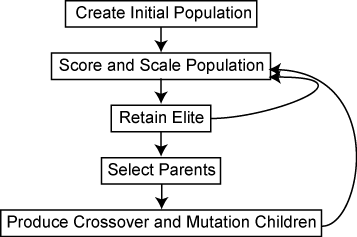
\includegraphics[width=0.4\linewidth]{genetic_diagram.png}
	\caption{Steps of a genetic algorithm \cite{mathworks_2012}}
\end{figure}

The approach we have used here is a decision version of the problem, with the additional logic of a binary search to arrive at the best possible result within the fixed time limit.

\subsubsection{Implementation}
This project uses the DEAP library\footnote{https://deap.readthedocs.io/en/master/index.html} which provides convenient wrappers for genetic algorithms. However, it should be noted that custom functions and logic have been used for the actual initiation, evaluation and mutation. The algorithm implemented is first defined in \cite{back2018evolutionary}. DEAP library documentation also provided the boilerplate code.

\subsubsection{Optimizations}
Due to the nature of genetic algorithms, convergence can be quite slow, and with large graphs there are tradeoffs to be made between speed and optimization. Some of the choices we made are listed below:

\begin{itemize}[topsep=\parskip]
  \item Reducing the number of generations and initial population size for larger graphs. The tradeoff here is lower accuracy, but it helps speed up computation.
  \item We keep a high bar for making a decision and only consider a positive result if it has converged. However, convergence rates can be slow and by the last generation if it hasn’t converged yet it can often be ambiguous. We consider that to be a negative outcome. This helps avoid false positives.
  \item A number of different mating and selection strategies offered by the DEAP library were explored and the ones which converged fastest were chosen.
\end{itemize}

\subsubsection{Algorithm Analysis}
Genetic algorithms boast several advantages. Due to its stochastic nature and initialization of a population of many points as opposed to one, genetic algorithms are robust against environments with large amounts of noise and can overcome local minima/maxima better than similar algorithms. They are also easy to understand/conceptualize due to their roots in evolutionary biology and clear real-life analogues. Lastly, genetic algorithms can be easily parellelized, allowing one to cut down on the total runtime of the algorithm.

The main weakness of genetic algorithms is that they are often computationally expensive and more time-consuming than other classes of algorithms. Additionally, there is no guarantee regarding the quality of the solution produced by a genetic algorithm. While its stochastic nature may allow it to avoid local optima, it can also make it unreliable and lead to low-quality solutions.

The time and space complexity of the algorithm is calculated as follows:
\vspace{-.5cm}
\begin{align*}
    \textnormal{Complexity} &= \textnormal{Cost of Binary Search} * \textnormal{Cost of the Genetic Algorithm}\\
    &= O(\log V) * \textnormal{Cost of the Genetic Algorithm}\\
    &= O(\log V) * [\textnormal{Cost of Initialization} + \textnormal{Number of Generations} * \textnormal{Population Size} * \\
    &(\textnormal{Cost of Selection} + \textnormal{Cost of Mating} + \textnormal{Cost of Mutating} + \textnormal{Cost of Evaluation})]\\
    &= O(\log V) * [(\textnormal{Population Size} * O(V) + \textnormal{Number of Generations} * \textnormal{Population Size} * \\
    &(O(E) + O(V) + O(1) + O(E))]\\
    &= O(\log V * \textnormal{Number of Generations} * \textnormal{Population Size} * (V + E))\\
\end{align*}

% $$
% \begin{aligned}
%     \textnormal{Complexity} &= \textnormal{Cost of Binary Search} * \textnormal{Cost of the Genetic Algorithm}\\
%     &= O(\log V) * \textnormal{Cost of the Genetic Algorithm}\\
%     &= O(\log V) * [\textnormal{Cost of Initialization} + \textnormal{Number of Generations} * \textnormal{Population Size} * \\
%     &(\textnormal{Cost of Selection} + \textnormal{Cost of Mating} + \textnormal{Cost of Mutating} + \textnormal{Cost of Evaluation})]\\
%     &= O(\log V) * [(\textnormal{Population Size} * O(V) + \textnormal{Number of Generations} * \textnormal{Population Size} * \\
%     &(O(E) + O(V) + O(1) + O(E))]\\
%     &= O(\log V * \textnormal{Number of Generations} * \textnormal{Population Size} * (V + E))\\
% \end{aligned}
% $$

\section{Empirical Evaluation}

% a detailed description of your platform (CPU, RAM, language, compiler, etc.), experimental procedure, evaluation criteria and obtained results (plots, tables, etc.). What is the lower bound on the optimal solution quality that you can drive from the results of your approximation algorithm and how far is it from the true optimum? How about from your branch-and-bound?

The branch and bound algorithm as well as the construction heuristic algorithm were tested on a a platform with an i7 8750H and 16GB RAM running Ubuntu 20.4. The simulated annealing algorithm was tested on a platform with an AMD Ruben 5900HX and 32GB RAM running Windows 11. The genetic algorithm was tested on a platform with an i7 12700H and 16GB RAM running Windows 11.

Each algorithm was run on 11 graph-based datasets. The algorithms were measured based on their total amount of wall-clock time to completion, the quality of the solution produced by the algorithm (i.e. the size of the vertex cover found, measured in nodes), and the relative error compared to the optimal solution. For the branch and bound algorithm, since the size of many of the datasets makes them prohibitively expensive/time-consuming to run to completion, the algorithm was cut off after a certain time threshold. Thus, in cases where the algorithm did not find an exact, optimal solution, we report the quality of the best solution it found, as well as the time it took to find that solution. These results can be found in Table \ref{table:alg_perf}.

\begin{table}[H]
	\caption{Algorithm Performance}
	\label{tab:freq}
	\begin{tabular}{|l|c|c|c|c|c|c|}
		\toprule
		&\multicolumn{3}{c|}{Branch and Bound}&\multicolumn{3}{c|}{Construction Heuristic}\\
		\midrule
		Dataset&Time(s)&VC Value&RelErr&Time(s)&VC Value&RelErr\\
		\midrule
		jazz&0.0054&159&0.063&0.0037&159&0.063\\
		karate&0.0011&14&0.00&0.0005&14&0.00\\
		football&0.0038&95&0.011&0.0014&95&0.011\\
		as-22july06&0.34&3303&0.00&0.21&3303&0.00\\
		hep-th&0.14&3943&0.0043&0.098&3943&0.0043\\
		star&0.27&7069&0.024&0.24&7069&0.024\\
		star2&0.24&4674&0.029&0.21&4674&0.029\\
		netscience&0.023&901&0.0022&0.017&901&0.0022\\
		email&0.024&604&0.017&0.015&604&0.017\\
		delaunay n10&0.016&733&0.043&0.012&733&0.043\\
		power&0.071&2226&0.010&0.051&2226&0.010\\
        \midrule
        &\multicolumn{3}{c|}{Simulated Annealing (avg of 10 runs)}&\multicolumn{3}{c|}{Genetic Algorithm (avg of 10 runs)}\\
        \midrule
        Dataset&Time(s)&VC Value&RelErr&Time(s)&VC Value&RelErr\\
		\midrule
        jazz&2.82&158.1&0.00063&81.03&162&0.025316\\
		karate&0.015&14.0&0.00&2.12&14&0\\
		football&0.48&94.0&0.00&16.22&97&0.031915\\
        as-22july06&7.12&16729.1&4.06&1158.76&21697&5.56887\\
		hep-th&4.98&5665.9&0.44&460.23&7259&0.848956\\
		star&6.27&10440.8&0.51&1080.91&10431&0.511301\\
		star2&5.14&12055.4&1.65&720.55&13217&1.909952\\
		netscience&4.68&986.3&0.097&1018.63&943&0.048943\\
		email&4.04&687.3&0.15&668.84&672&0.131313\\
		delaunay n10&5.17&768.3&0.092&1042.15&772&0.098151\\
		power&5.91&3108.2&0.41&790.75&4094&0.858375\\
		\bottomrule
	\end{tabular}
\label{table:alg_perf}
\end{table}

Additionally, we provide the Qualified Runtime for various solution qualities (QRTDs), Solution Quality Distributions for various run-times (SQDs), and Box plots for running times for both of the local search algorithms in Appendix \ref{sec:local}.

\section{Discussion}

% a comparative analysis of how different algorithms perform with respect to your evaluation
% criteria, or expected time complexity, etc
Firstly, the results of the branch and bound algorithm and the construction heuristic algorithm invite comparison, as the quality of the solutions produced by the two for each dataset are equivalent. In other words, we can infer that for the vast majority of the datasets tested in our evaluation, the branch and bound algorithm was unable to finish before timing out, and it was unable to find a better solution than the one produced by the heuristic. As a result, the branch and bound algorithm produced solutions no better than those produced by the heuristic while also incurring greater runtimes.

Secondly, we can compare the results of the two local search algorithms: simulated annealing and the genetic algorithm. Between the two, simulated annealing led to a high quality solution on nearly every dataset (except for the netscience and email datasets) and took dramatically less time to finish on all datasets, resulting in a speedup of over 10x or even 100x over the genetic algorithm. The divide between these two algorithms is also reflected in the plots in Appendix \ref{sec:local}. For example, in Figures 3 and 9, it is clear that simulated annealing runs reach a viable solution much more quickly than genetic algorithm runs, while in Figures 4 and 10, it is shown that simulated annealing runs produce solutions of higher quality than those of genetic algorithm runs given the same amount of time. These results align with expectations considering the differences in the theoretical complexities of both algorithms as described in their respective sections. Based on these results, we can conclude that simulated annealing is the local search algorithm with the highest overall performance of the algorithms we tested.

Finally, we note that there is a clear gap in the performance between the branch and bound/heuristic methods and the local search methods. The former produce solutions of higher quality on most (but not all) datasets (exceptions being the jazz and football datasets, on which the simulated annealing algorithm performed best), and they achieve much faster runtimes on all datasets.


\section{Conclusion}
Based on the results that we found, we conclude that the construction heuristic algorithm implemented here -- the \textit{Greedy Independent Cover (GIC)} algorithm proposed by Halld\'{o}rsson and Radhakrishnan \cite{Hall97} -- is the overall best and most viable approach towards solving the Minimum Vertex Cover problem out of the four approaches we tested. The approach should be preferred unless an exact solution is needed, in which case the branch and bound algorithm may be preferable (though possibly unfeasible).

There are several improvements to this project we could consider for future work. For example, we could test additional types of local search algorithms in addition to the ones presented here, such as a "hill climbing" algorithm. We could also work on optimizing the lower bound of the branch and bound algorithm in order to improve its performance and ideally produce substantively different results compared to the construction heuristic. Finally, we acknowledge that due to time constraints, the experiments for the various algorithms were conducted on different machines which may have adversely impacted the results; however we believe that the differences in computing power between the environments were small enough that they would not have changed the overall rankings/findings. A future study on algorithms for solving the Minimum Vertex Cover problem would ideally involve all experiments being run on the same machine to ensure consistency and validity of results. 

%%
%% The acknowledgments section is defined using the "acks" environment
%% (and NOT an unnumbered section). This ensures the proper
%% identification of the section in the article metadata, and the
%% consistent spelling of the heading.


\begin{acks}
We would like to thank Professor Wei Xu for teaching this course (CSE6140), as well as all of the TAs that have helped us throughout the semester.
\end{acks}

%%
%% The next two lines define the bibliography style to be used, and
%% the bibliography file.
\bibliographystyle{ACM-Reference-Format}
\bibliography{sample-base.bib}

\appendix

\newpage \section{Local Search Plots}\label{sec:local}

\begin{figure}[h]
	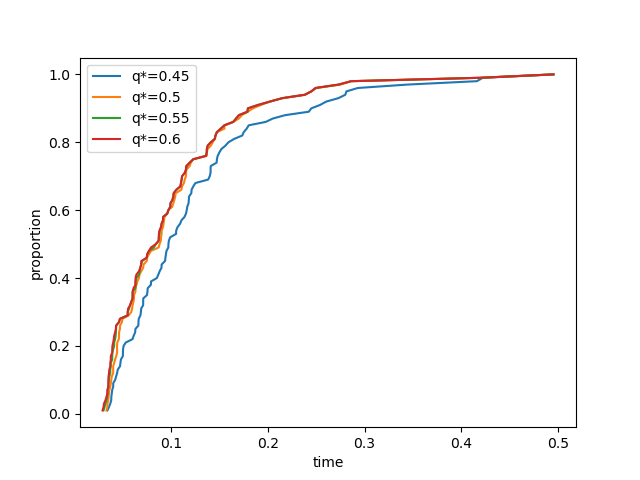
\includegraphics[width=\linewidth]{power_QRTD_LS1.png}
	\caption{QRTD of Power, Simulated Annealing}
\end{figure}


\begin{figure}[h]
	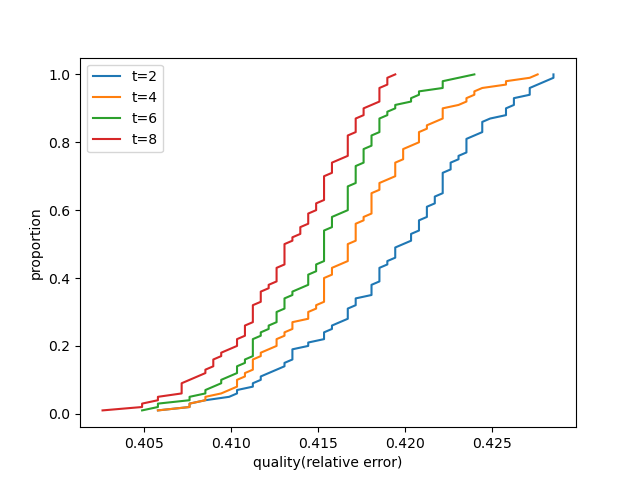
\includegraphics[width=\linewidth]{power_SQD_LS1.png}
	\caption{SQD of Power, Simulated Annealing}
\end{figure}

\begin{figure}[h]
	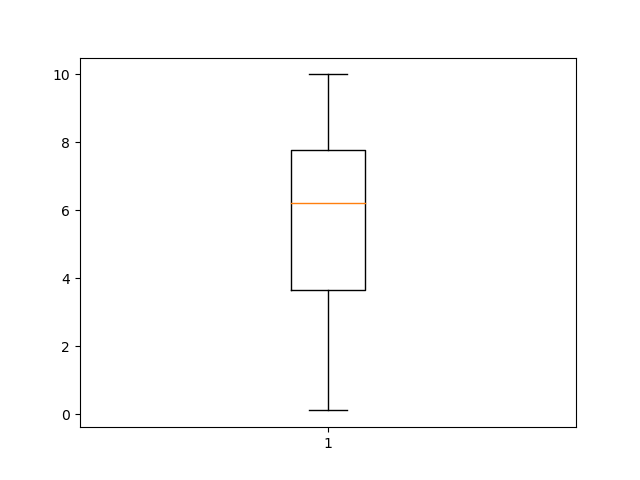
\includegraphics[width=\linewidth]{power_boxplot_LS1.png}
	\caption{boxplot of Power, Simulated Annealing}
\end{figure}


\begin{figure}[h]
	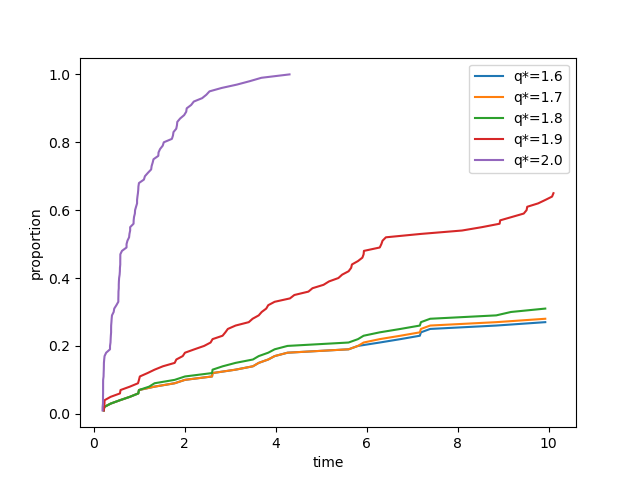
\includegraphics[width=\linewidth]{star2_QRTD_LS1.png}
	\caption{QRTD of Star2, Simulated Annealing}
\end{figure}


\begin{figure}[h]
	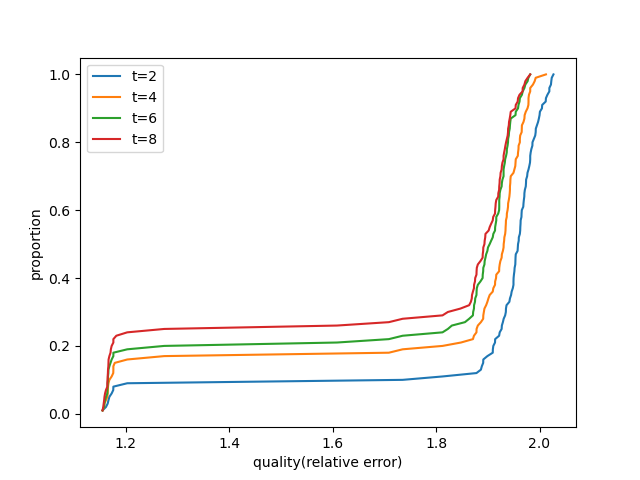
\includegraphics[width=\linewidth]{star2_SQD_LS1.png}
	\caption{SQD of Star2, Simulated Annealing}
\end{figure}

\begin{figure}[h]
	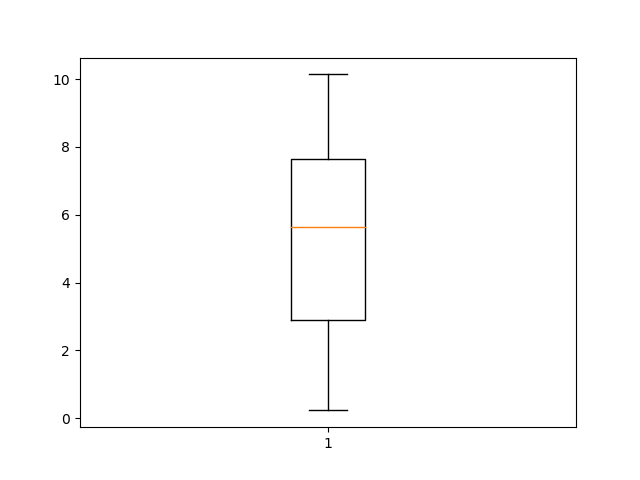
\includegraphics[width=\linewidth]{star2_boxplot_LS1.png}
	\caption{boxplot of Star2, Simulated Annealing}
\end{figure}

% Local Search 2 plots

\begin{figure}[h]
	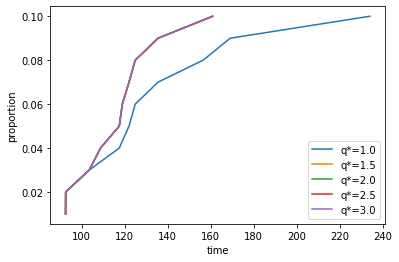
\includegraphics[width=\linewidth]{power_LS2_QRTD.png}
	\caption{QRTD of Power, Genetic Algorithm}
\end{figure}


\begin{figure}[h]
	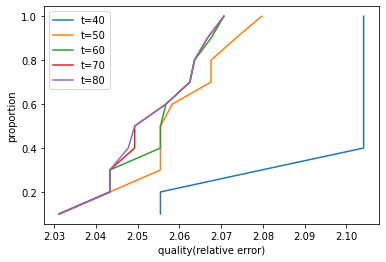
\includegraphics[width=\linewidth]{power_LS2_SQD.png}
	\caption{SQD of Power, Genetic Algorithm}
\end{figure}

\begin{figure}[h]
	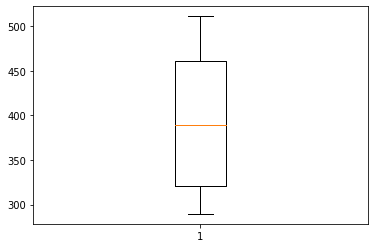
\includegraphics[width=\linewidth]{power_LS2_box.png}
	\caption{boxplot of Power, Genetic Algorithm}
\end{figure}


\begin{figure}[h]
	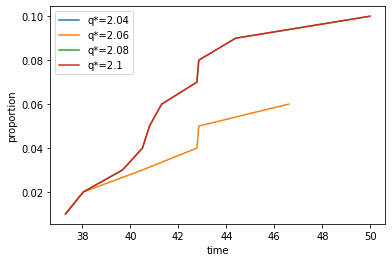
\includegraphics[width=\linewidth]{star2_LS2_QRTD.png}
	\caption{QRTD of Star2, Genetic Algorithm}
\end{figure}


\begin{figure}[h]
	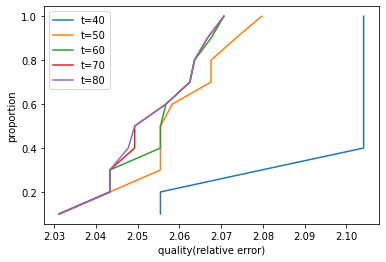
\includegraphics[width=\linewidth]{star2_LS2_SQD.png}
	\caption{SQD of Star2, Genetic Algorithm}
\end{figure}

\begin{figure}[h]
	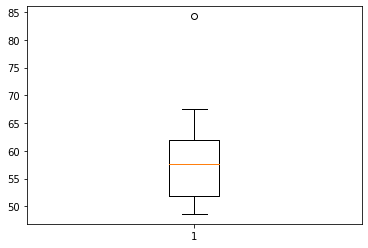
\includegraphics[width=\linewidth]{star2_LS2_box.png}
	\caption{boxplot of Star2, Genetic Algorithm}
\end{figure}

\end{document}
\endinput
%%
%% End of file `sample-acmlarge.tex'.
